\documentclass{beamer}

% The ams packages are required to insert any mathematical symbols that you may require
\usepackage{amsfonts}
\usepackage{amssymb}
\usepackage{amsmath}
\usepackage{amsthm}
% This package is used for embedding things like PDFs and JPEGs into your document
\usepackage{graphicx}
% This package is used for drawing pictures (such as trees)
\usepackage{tikz}
\usetikzlibrary{arrows,automata}
% These packages are used for adding pseudo-code to your document
\usepackage{algorithm2e}
\usepackage{algorithmic}
% This package is for if you require an appendix
\usepackage{appendix}

\usepackage{datetime}
\usepackage{fancyhdr}
\usepackage{semantic}
\usepackage[noload]{qtree}
\usepackage{comment}
\usepackage{pdflscape}
\usepackage{graphicx}
\usepackage{moreverb}
\usepackage{caption}
\usepackage{url}
\usepackage{layout}
\usepackage{subfig}
\usepackage{lineno}
\usepackage{bm}


\usetheme{Warsaw}
\title[Talking about things]{I'm making a presentation!}

\author{Tim Jones}

\institute{Some room in the maths building I guess.}
\date{\today}

\begin{document}

\begin{frame}{Introduction}
\titlepage
\end{frame}

\begin{frame}{The Problem}
\begin{itemize}
\item Modelling humans is hard.
\pause \item Twitter, emails, network logs
\pause \item Being able to spot anomalies would have great applications for spotting botnets, suspicious activity, etc
\pause \item Several assumptions have been made, but no objective studies
\end{itemize}
\end{frame}

\begin{frame}{Candidate Models}
\begin{itemize}
\item The Poisson process
\pause \item The inhomogeneous Poisson process
\pause \item The Markov-modulated Poisson process
\pause \item A discrete-time interlude
\pause \item The Markov-modulated renewal process
\end{itemize}
\end{frame}

\begin{frame}{But first...}
Preliminaries; the Markov Chain (DTHMM)
\begin{itemize}
\pause \item Arbitrary state space $S$ - here it will be discrete
\pause \item Transition matrix $\Pi = (\pi_{ij})_{(i,j) \in S^2}$
\pause \item Initial probability vector $\bm{\delta} = (\delta_s)_{s \in S}$
\pause \item Start in a state determined by $\bm{\delta}$, then hop from sate to state according to the probabilities in $\Pi$
\end{itemize}
\end{frame}

\begin{frame}{But first...}
The Continuous Time Markov Chain (CTMC)
\begin{itemize}
\pause \item Similar to before, but in continuous time
\pause \item Transition rate matrix $Q = (q_{ij})_{(i,j) \in S^2}$
\pause \item Remain in state $i$ for an $\mathrm{Exp}(-q_{ii})$ amount of time, then hop to state $j$ with probability $\frac{-q_{ii}}{q_{ij}}$
\end{itemize}
\end{frame}


\begin{frame}{But first...}
The Poisson Process
\begin{itemize}
\pause \item A CTMC where $S = \mathbb{N}$, $\delta_0 = 1$ and,
\begin{align*}
\forall i \in S \quad q_{i,i+1} &= \lambda \\
q_{i,i} &= -\lambda
\end{align*}
\pause \item Crucially, inter-arrival times are exponential
\end{itemize}
\end{frame}

\begin{frame}{But first...}
Hidden Markov Models
\begin{itemize}
\pause \item We believe there's a Markov Chain somewhere, but we can't see it
\pause \item The chain hops between states
\pause \item With each transition, an emission is made
\pause \item The distribution of emissions depends on the state
\pause \item Can be either discrete or continuous time or emissions, or even state
\end{itemize}
\end{frame}

\begin{frame}{But first...}
The Markov Modulated Poisson Process
\begin{itemize}
\pause \item A Poisson process whose rate varies randomly with time
\pause \item A form of continuous time, discrete state, continuous emission Hidden Markov Model in which the emissions are Poisson processes
\pause \item No I am not crazy
\pause \item Suspected to be a good model, but no objective studies had been performed until now
\end{itemize}
\end{frame}

\begin{frame}{But first...}
Fitting Hidden Markov Models
\begin{itemize}
\pause \item Baum-Welch and Viterbi
\pause \item Baum-Welch estimates the underlying parameters by expectation-maximisation
\pause \item Viterbi estimates the most likely state sequence given the underlying parameters by dynamic programming
\pause \item Baum-Welch already exists for the MMPP, but no implementation of Viterbi existed until now
\pause \item A perfect MMPP Viterbi is \emph{really} hard, but a very close approximation for most practical cases has been used
\end{itemize}
\end{frame}

\begin{frame}{If you only have a hammer...}
Fitting the MMPP
\begin{itemize}
\pause \item Applying these algorithms to the data produces fairly sane-looking results
\end{itemize}
\includegraphics[width = \textwidth]{./images/fit_mmpp2.png}
\end{frame}

\begin{frame}{If you only have a hammer...}
Fitting the MMPP
\begin{itemize}
\pause \item The parameters are questionable
\begin{align*}
(\lambda_1,\lambda_2,\lambda_3) &= (0.0289,1.28,15.5)\\
S &= \{\lambda_1,\lambda_2,\lambda_3\}\\
Q &= \bordermatrix{      & \lambda_1 & \lambda_2 & \lambda_3\cr
                \lambda_1 & -0.123 & 0.120 & 0.004 \cr
                \lambda_2 & 0.441 & -1.09 & 0.648 \cr
                \lambda_3 & 0.00 & 5.25 & -5.25 \cr
			}\\
\bm{\delta} &= (1.00,0.00,0.00)
\end{align*}
\pause \item I don't go to sleep every 2 hours or so...
\pause \item Why only use 3 states?
\end{itemize}
\end{frame}

\begin{frame}{If you only have a hammer...}
Fitting a better MMPP
\begin{itemize}
\pause \item Use the Bayesian Information Criterion
$$
BIC = -2 \ln L + k \ln n
$$
\pause \item 4 states give the best model
\end{itemize}
\end{frame}

\begin{frame}{If you only have a hammer...}
More sane results!

\includegraphics[width = \textwidth]{./images/fit_mmpp3.png}
\end{frame}

\begin{frame}{...is everything a nail?}
The Kolmogorov-Smirnov test
\begin{itemize}
\pause \item How far apart are these two densities?
\pause \item In an MMPP, we'd expect most inter-arrival times to be Exponential
\pause \item Testing a null hypothesis of expovariance against the observed per-state inter-arrival times yields...
\pause
\begin{align*}
p_1 &< 10^{-5} \\
p_2 &< 10^{-5} \\
p_3 &< 10^{-5} \\
p_4 &< 10^{-5}
\end{align*}
\pause \item Well so much for that, then...
\end{itemize}
\end{frame}

\begin{frame}{An alternative tool}
An Exponential DTHMM
\begin{itemize}
\pause \item Assume only single inter-arrival transitions
\pause \item Ignore link between transition probabilities and observed inter-arrival times
\pause \item Still clustering Exponentially distributed inter-arrivals into Exponentially distributed time sums, so still serves as a reasonable heuristic
\end{itemize}
\end{frame}

\begin{frame}{An alternative tool}
\begin{itemize}
\item Yet more sanity occurs
\end{itemize}
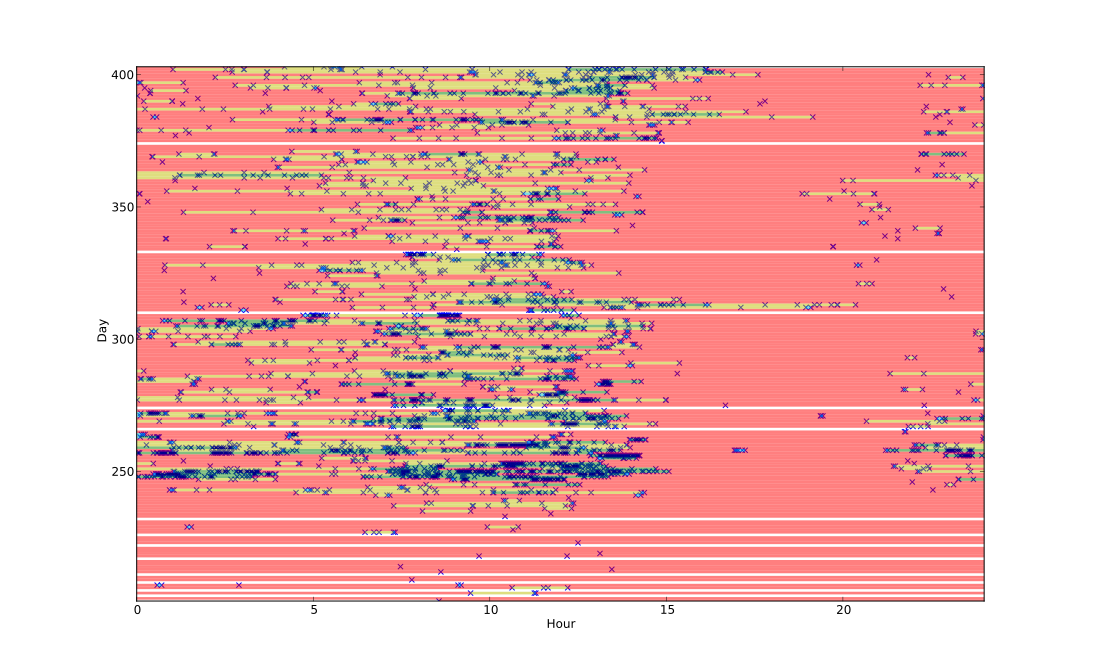
\includegraphics[width = \textwidth]{./images/fit_dthmm1.png}
\end{frame}

\begin{frame}{Not alternative enough}
Kolmogorov and Smirnov strike again
\begin{itemize}
\pause \item One $p$-value of 0.03
\pause \item All others below $10^{-7}$
\pause \item We can conclude that the emissions cannot be clustered into some small number of exponentially distributed subsets
\pause \item So what are they?
\end{itemize}
\end{frame}

\begin{frame}{Plot some graphs}
\centering
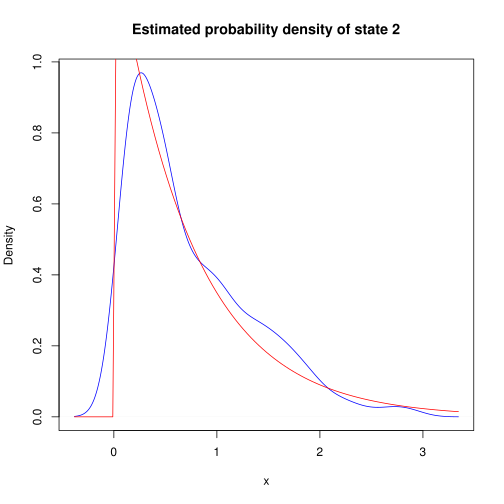
\includegraphics[height = 0.8\textheight]{./images/density_mmpp1_state2.png}
\end{frame}

\begin{frame}{Lognormality is humanity}
DTHMM with lognormal emissions
\begin{itemize}
\pause \item If $X$ is normally distributed, then $\ln (X)$ is lognormally distributed
\pause \item Allows for light heads and heavy tails, exactly what we neeed
\pause \item Take the logs of the inter-tweet times, fit a DTHMM with normal emissions
\pause \item The $BIC$ tells us that 3 states is the way to go
\pause
\begin{align*}
S &= \{1,2,3\}\\
(\mu_1, \mu_2, \mu_3) &= (-3.33, -1.33, 2.34)\\
(\sigma_1, \sigma_2, \sigma_3) &= (1.47, 1.86, 0.366)\\
\bm{\delta} &= (0,1,0)\\
\Pi &= 
\left(
	\begin{matrix}
     0.926 & 0.069 & 0.006 \\
     0.047 & 0.906 & 0.047 \\
     0.000 & 0.865 & 0.135
	\end{matrix}
\right)
\end{align*}
\end{itemize}
\end{frame}

\begin{frame}{Lognormality is humanity}
Looks sane, passes all the Kolmogorov-Smirnov tests
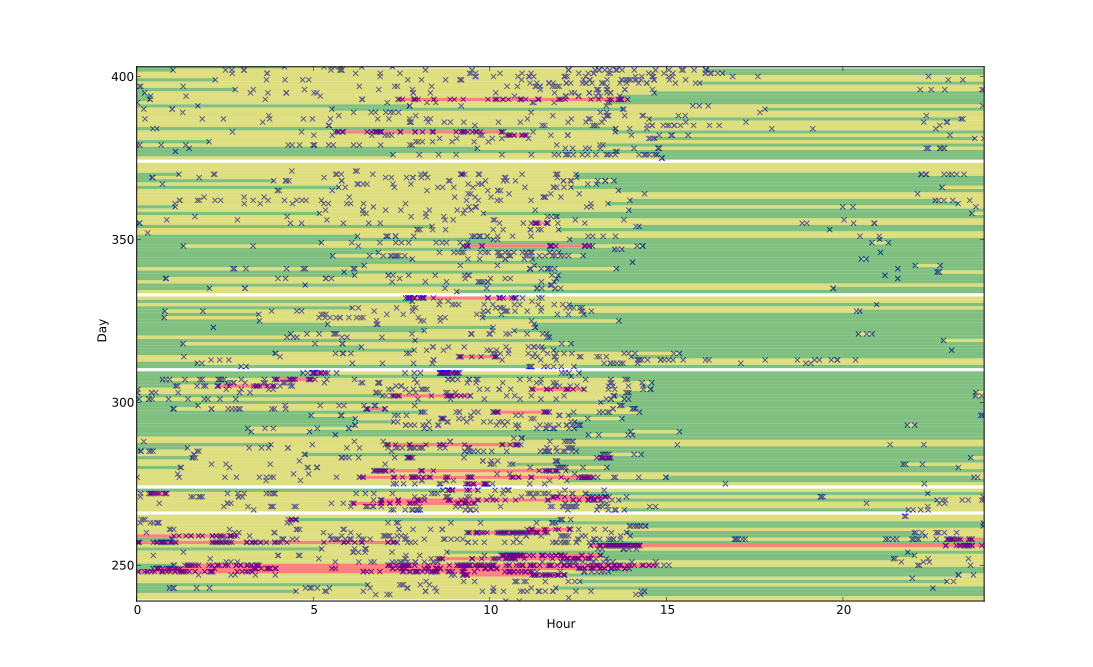
\includegraphics[width = \textwidth]{./images/fit_dthmm2.png}
\end{frame}

\begin{frame}{At last!}
DTHMM with lognormal emisssions
\begin{itemize}
\pause \item This is how people probably behave
\pause \item Could be extended to the Markov Modulated Renewal process
\pause \item Spot anomalies as and when they happen
\pause \item Questions?
\end{itemize}
\end{frame}
\end{document}